\documentclass{article}
\usepackage[margin=1in]{geometry}
\usepackage{amsmath}
\usepackage{listings}
\usepackage{color}
\usepackage{graphicx}
\usepackage{blkarray}
\usepackage{multirow}

\definecolor{dkgreen}{rgb}{0,0.6,0}
\definecolor{gray}{rgb}{0.5,0.5,0.5}
\definecolor{mauve}{rgb}{0.58,0,0.82}

\lstset{frame=tb,
  language=Python,
  aboveskip=3mm,
  belowskip=3mm,
  showstringspaces=false,
  columns=flexible,
  basicstyle={\small\ttfamily},
  numbers=none,
  numberstyle=\tiny\color{gray},
  keywordstyle=\color{blue},
  commentstyle=\color{dkgreen},
  stringstyle=\color{mauve},
  breaklines=true,
  breakatwhitespace=true,
  tabsize=3
}

\begin{document}
\begin{titlepage}
	\setlength{\parindent}{0pt}
	\large

\vspace*{-2cm}

University of Waterloo \par
Econ 424 \par
2023-10-21 \par
\vspace{0.05cm}
Anonymized Usernmae: IJustWannaPass
\vspace{0.2cm}

{\huge Prediction Competition \# 4 \par}
\hrule

\vspace{1cm}
\textbf{Q1)} To solve this problem, I used a variation of boosting. Due to the fact that across k feature space the data could still not be accurately linearly estimated (as shown in Q2), what I did was split the data into buckets. Each bucket would have its own boosted model trained on the data in the bucket. Then I would use a boosted model to create a rough estimate for the price, and determine what bucket to use to get a more accurate measure. This model has the following traits for the training data:
\[ MSE = 0.06275 \]
\[ R^2 = 0.82178 \]

\textbf{Q2)} Below is the graph to show how the prediction accuracy verifies with price. The data was partitioned into 5 parts (by price), and the MSE was calculated for each section:
\begin{center}
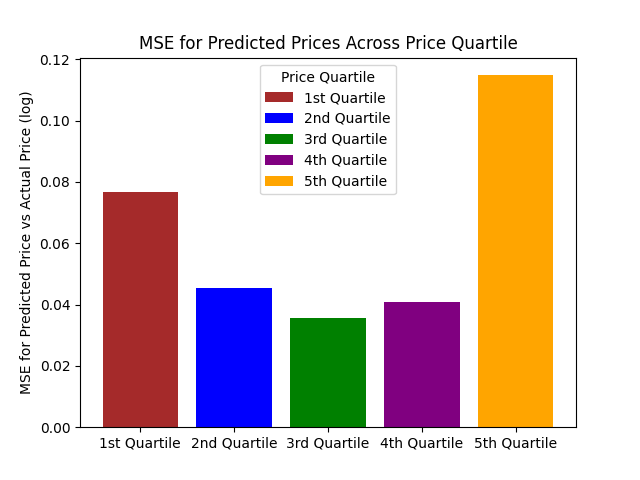
\includegraphics[width=0.8\textwidth]{g1.png}
\end{center}
As we can see, the more expensive the cars are, the worse our predictions get. Therefore if we are writing predictions for expensive cars (like in pc5) we need to be careful of the data being used.
\newpage
\textbf{Q4)} To solve Q1 chatGPT was given the prompt: 
\begin{verbatim}
  Given a training set of car features, how can I use python to most accurately predict a cars value?
\end{verbatim}
chatGPT provided the following response:
\begin{verbatim}
Predicting a car's value is a regression problem, and you can use various machine learning techniques in Python to achieve accurate predictions. Here's a general outline of the steps you can follow:

Data Collection: Gather a dataset containing information about various car features (e.g., make, model, year, mileage, fuel efficiency, horsepower, etc.) and their corresponding values or prices.

Data Preprocessing:

a. Data Cleaning: Handle missing values and outliers in the dataset.

b. Feature Selection: Choose relevant features that have a significant impact on a car's value.

c. Data Encoding: Convert categorical features into numerical representations using techniques like one-hot encoding.

d. Data Splitting: Split the dataset into a training set and a testing set to evaluate the model's performance.

Feature Scaling: Normalize or standardize numerical features to ensure that all features have the same scale. This helps the machine learning algorithms perform better.

Model Selection: Choose a regression algorithm. Common choices include Linear Regression, Decision Trees, Random Forest, Support Vector Regression, or Gradient Boosting.

Model Training: Train the selected model on the training data.

Model Evaluation: Use the testing set to evaluate the model's performance. Common regression metrics include Mean Absolute Error (MAE), Mean Squared Error (MSE), and R-squared (R2) score.

Hyperparameter Tuning: Depending on the model you choose, you may need to tune hyperparameters to improve its performance. Techniques like cross-validation can help with this.

Deployment: Once you are satisfied with the model's performance, you can deploy it to make predictions on new, unseen data.

Continuous Monitoring and Maintenance: Keep an eye on your model's performance and update it as new data becomes available.

Remember that the choice of features, data quality, and the model you select will have a significant impact on the prediction accuracy. It's often an iterative process where you experiment with different models and feature engineering techniques to improve the results.
\end{verbatim}
\newpage
To solve Q2 chatGPT was given the prompt:
\begin{verbatim}
   How can we determine how well our model predicts on different ranges of car prices?
\end{verbatim}
chatGPT provided the following response: \\\\
\begin{verbatim}
To determine how well your model predicts on different ranges of car prices, you can perform the following steps:

Define Price Ranges: First, define the price ranges or bins into which you want to categorize the car prices. For example, you might create bins such as "Affordable," "Moderate," and "Luxury" or specify numerical ranges like "0-10,000," "10,000-20,000," "20,000-30,000," and so on.

Group Data: Group the test data into these defined price ranges. You can use pandas in Python to do this.

Predict Prices: Use your trained model to make predictions for each data point in the testing set.

Evaluate Accuracy: Calculate accuracy metrics for each price range. You can use metrics like Mean Absolute Error (MAE), Mean Squared Error (MSE), R-squared (R2), or custom metrics specific to your application. Calculate these metrics separately for each price range to understand how well your model performs in each category.

By evaluating the model's performance on different price ranges, you can gain insights into how well your model predicts for cars in various price categories. This analysis can help you identify whether the model excels in certain price ranges and where it might need improvement.
\end{verbatim}
\end{titlepage}
\textbf{Code for Q1:}
\begin{lstlisting}
import matplotlib.pyplot as plt
import numpy as np
import pandas as pd
import xgboost as xgb
import warnings
from pandas.util import hash_pandas_object

warnings.filterwarnings("ignore")
from sklearn.model_selection import train_test_split
from sklearn.neighbors import KNeighborsClassifier

# Read in the data
data = pd.read_csv("Econ424_F2023_PC4_training_data_large.csv", low_memory=False)

# Keep only the most relevant stats
data = data.loc[:,
       data.columns.intersection(['price', 'model_name', 'mileage', 'daysonmarket', 'owner_count', 'year'])]
# If owner_count is empty assume its 0
data["owner_count"] = data["owner_count"].fillna(0)
# Drop empty columns
data.dropna(inplace=True)
# Standardize results
data["price"] = data["price"].map(lambda x: np.log(x))
data["mileage"] = data["mileage"].map(lambda x: np.log(int(x) + 1))

# ===================== Data Processing =====================
# assign each value to a dict
modelDict = {}


def classify(model):
    if model not in modelDict:
        modelDict[model] = len(modelDict)


data.apply(lambda x: classify(x['model_name']), axis=1)
data["model_name"] = data["model_name"].map(lambda x: modelDict[x])

# We will now define 3 buckets dependent on the price of the car, such that if we estimate a car to be in a specific
#  range we will use the bucket estimate instead of the overall estimator.
data.sort_values(by=['price'], inplace=True, ignore_index=True)

numberOfBuckets = 11
numberOfEntries = len(data)
markers = [data.iloc[0, 0]]
adjustment = np.abs((data.iloc[0, 0] - data.iloc[numberOfEntries - 1, 0]) / 14)
for i in range(1, numberOfBuckets + 1):
    if i == numberOfBuckets:
        markers.append(data.iloc[numberOfEntries - 1, 0])
    else:
        markers.append(data.iloc[int(i * numberOfEntries / numberOfBuckets), 0])

# We will then train classifiers with data a little past each marker
modelArr = []
for bucket in range(0, numberOfBuckets):
    if bucket == numberOfBuckets - 1:
        slice = data[(data['price'] > markers[bucket] - adjustment) & (data['price'] <= markers[bucket + 1])]
    elif bucket == 0:
        slice = data[(data['price'] >= markers[bucket]) & (data['price'] <= markers[bucket + 1] + adjustment)]
    else:
        slice = data[
            (data['price'] > markers[bucket] - adjustment) & (
                    data['price'] <= markers[bucket + 1] + adjustment)]

    innerModel = xgb.XGBRegressor(n_estimators=500, max_depth=4, eta=0.1, subsample=0.7, colsample_bytree=0.8)
    x = slice.iloc[:, 1:]
    y = slice.iloc[:, 0]
    innerModel.fit(x, y)
    modelArr.append(innerModel)

print(markers)


# ===================== Data Testing =====================

def getModelName(modelName):
    if modelName in modelDict:
        return modelDict[modelName]
    return 0


# Read in the test data and modify the data
test = pd.read_csv("Econ424_F2023_PC4_test_data_without_response_var.csv", low_memory=False)
test["owner_count"] = test["owner_count"].fillna(0)
test = test.interpolate()
test = test.loc[:,test.columns.intersection(['model_name', 'mileage', 'daysonmarket', 'owner_count', 'year'])]
test["model_name"] = test["model_name"].map(lambda x: getModelName(x))
test["mileage"] = test["mileage"].map(lambda x: np.log(int(x) + 1))

# Start by predicting using a regular classifier, based of results use a more specific classifier
baseLine = xgb.XGBRegressor(n_estimators=500, max_depth=4, eta=0.1, subsample=0.7, colsample_bytree=0.8)
x = data.iloc[:, 1:]
y = data.iloc[:, 0]
baseLine.fit(x, y)
prediction_base = baseLine.predict(test)
test["predicted_base_price"] = prediction_base
test['New_ID'] = test.index


pred = {}
# Using the old predictions, use the buckets to predict again
for bucket in range(0, numberOfBuckets):
    print(bucket)
    if bucket == numberOfBuckets - 1:
        slice = test[test['predicted_base_price'] > markers[bucket]]
    elif bucket == 0:
        slice = test[test['predicted_base_price'] <= markers[bucket + 1]]
    else:
        slice = test[
            (test['predicted_base_price'] > markers[bucket]) & (
                    test['predicted_base_price'] <= markers[bucket + 1])]

    slice.reset_index()
    loctest = slice.iloc[:, 0:-2]
    loctest.reset_index()
    predicted = modelArr[bucket].predict(loctest)

    for idx in range(0, len(predicted)):
        key = slice.iloc[idx, -1]
        pred[key] = predicted[idx]



# ===================== Export Model =====================

test["predicted_spec_price"] = test.apply(lambda x: pred[x.loc['New_ID']], axis=1)
val = test["predicted_spec_price"]

f = open('predictions.csv', 'w')
for estimate in val:
    f.writelines(str(estimate) + ",\n")

\end{lstlisting}
\end{document}